

\documentclass[11pt,pdf,hyperref={unicode}]{beamer}
\beamertemplatenavigationsymbolsempty

\setbeamertemplate{blocks}[rounded=true, shadow=true]
\setbeamertemplate{footline}[page number]
\usepackage{multicol}

\usefonttheme{serif}

\usepackage[utf8]{inputenc}
\usepackage[russian]{babel}
\usepackage{amsmath,mathrsfs,mathtext}
\usepackage{graphicx, epsfig}
\usepackage{subfloat}
\usepackage{wrapfig}
\usepackage{multicol}
\usepackage[caption=false]{subfig}
\usetheme{Warsaw}%{Singapore}%{Warsaw}%{Warsaw}%{Darmstadt}
\usecolortheme{sidebartab}

%----------------------------------------------------------------------------------------------------------
\title[\hbox to 56mm{Прогнозирование химических реакций \hfill\insertframenumber\,/\,\inserttotalframenumber}]
{Прогнозирование количественного выхода химических реакций с помощью графовых нейронных сетей}
\author[Гунаев Р.\ Г.]{\Large Гунаев Руслан Гуламович}
\institute{ Московский физико-технический институт\\
Факультет управления и прикладной математики\\
Кафедра интеллектуальных систем\\
~\\
Консультант \ Ф. Никитин\\
}
\date{\footnotesize{\emph{Курс:} Численные методы обучения по прецедентам\par (практика, В.\,В. Стрижов)/Группа 774, весна 2020}}
%----------------------------------------------------------------------------------------------------------
\begin{document}
%----------------------------------------------------------------------------------------------------------
\begin{frame}
%\thispagestyle{empty}
\titlepage
\end{frame}
%-----------------------------------------------------------------------------------------------------
\begin{frame}{Прогнозирование количественного выхода химической реакции}
%\begin{block}{Актуальность исследования}
%\end{block}

\begin{block}{Цель}
    Предложить графовые нейронные сети для решения задачи регрессии на множестве молекулярных графов для прогнозирования количественного выхода химической реакции, используя экспертные знания.
    \end{block}
    
\begin{alertblock}{Определение}
\footnotesize{\alert{Молекулярный граф} --  связный неориентированный граф, находящийся во взаимно-однозначном соответствии со структурной формулой химического соединения таким образом, что вершинам графа соответствуют атомы молекулы, а рёбрам графа — химические связи между этими атомами.

\alert{Экспертные} знания -- информация о
\alert{химичических связях}(одинарная, двойная, тройная, ароматическая) и о \alert{свойствах атомов}(степень, явная валентность, гибридизация, неявная валентность, ароматичность, неявность и т.д.).}
\end{alertblock}
 
\end{frame}

\begin{frame}{Продукт и реагенты химической реакции}
%Пример \text{SMILES}: \footnotesize{CC(=O)c1ccco1.Nc1ccc(Cl)c(Cl)c1>CC(C)=O.Cl.O.O=N[O-].[Na+]>CC(=O)c1ccc(-c2ccc(Cl)c(Cl)c2)o1}%
\begin{figure}
\subfloat[Продукт]{
    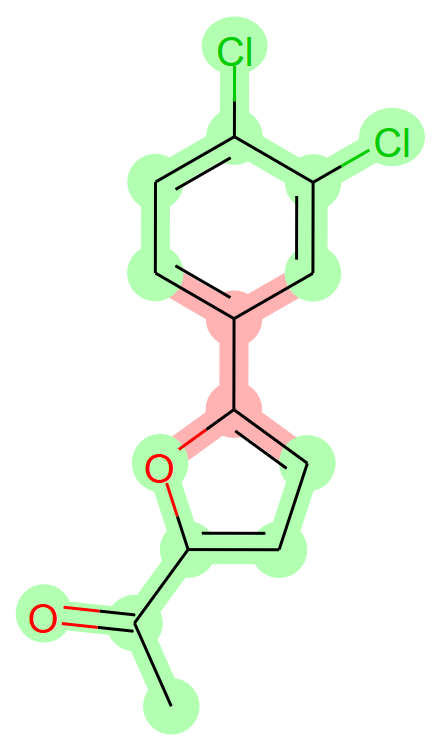
\includegraphics[width=0.3\textwidth]{product.jpg}}
\subfloat[Реагенты]{
    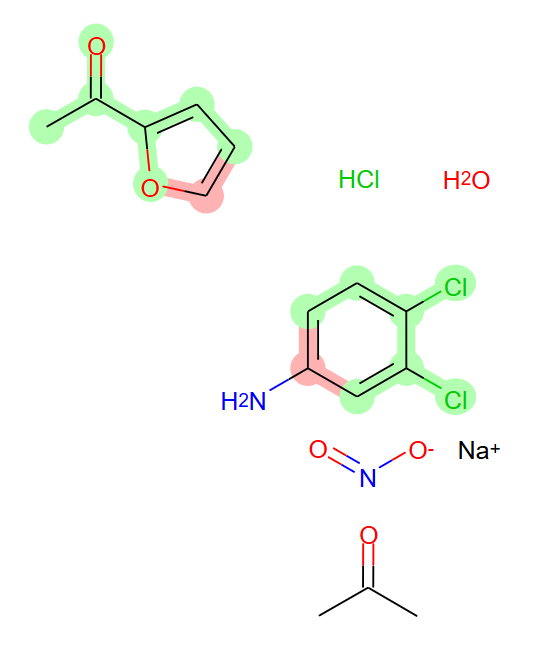
\includegraphics[width=0.5\textwidth]{reac.jpg}}
\end{figure}
\end{frame}

\begin{frame}{Описание данных}
\begin{block}{База реакций}
\begin{enumerate}
    \item 1 млн. реакций в формате \text{SMARTS}
    \item Разделены продукты и реагенты
    \item Известен основной продукт
    \item Для $20\%$ реакций известен количественный выход основного продукта
\end{enumerate}
\end{block}
\begin{alertblock}{Справка}
\footnotesize{
\alert{SMILES} -- язык, позволяющий однозачно закодировать молекурлярный граф строкой символов \text{ASCII}, \text{SMARTS} -- поднастройка \text{SMILES}.
\alert{Реагент} -- вещество, участвующее в химической реакции.

\alert{Продукт} -- вещество, которое поменяло свое строение в результате реакции.

\alert{Основной продукт} -- молекула, включающая в себя наибольшее количество атомов среди всех продуктов реакции.

}
\end{alertblock}
\end{frame}


\begin{frame}{Литература}
    \bibliographystyle{plainnat}
    \nocite{*}
    \bibliography{literature} 
\end{frame}

%----------------------------------------------------------------------------------------------------------

%----------------------------------------------------------------------------------------------------------


%----------------------------------------------------------------------------------------------------------

\begin{frame}{Постановка задачи}

\begin{block}{Выборка}
$X = \{g_i, y_i\}_{i = 1}^N,$ $g_i \in G$ -- множество входных молекулярных графов, $y_i$ -- выход реакции.
\end{block}
\begin{block}{Модель}
$$
f(g, \mathbf{W}):~G\times \Omega \rightarrow \mathbb{R},
$$
$\Omega$ -- пространство параметров модели.
\end{block}
\begin{block}{Задача}
Найти $\mathbf{W}^*$ такую, что 
$$
\mathbf{W^*} = \text{arg}\min_{\mathbf{W} \in \Omega}\dfrac{1}{N}\sum_{i = 1}^N \|y_i - f(g_i, \mathbf{W})\|_2^2.
$$
\end{block}

    
\end{frame}

\begin{frame}{Архитектура модели}

\begin{multicols}
\normalsize

\begin{enumerate}
    \item Инициализация векторных представлений вершин молекулярного графа
    \item Графовая сверточная нейронная сеть
    \item Агрегация графа
    \item Полносвязная нейронная сеть
    \item Получение выхода реакции
\end{enumerate}
\columnbreak
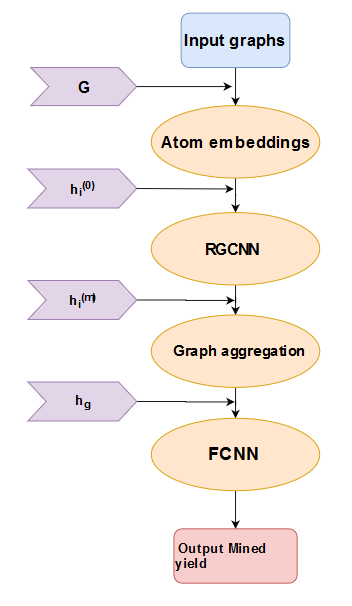
\includegraphics[width=0.4\textwidth]{model.jpg}

\end{multicols}

\end{frame}

\begin{frame}{Инициализация вершин молекулярного графа}

\begin{block}{Эмбеддиниги}
$$\mathbf{h}_{ik}^{(0)} = W^k_i,$$ $W^k$ -- матрица эмбеддинга для $k$-го категориального признака, $i$ -- номер столбца матрицы, верхний индекс $\mathbf{h}_{ik}^{(0)}$ означает, что вектор на нулевом слое.
\end{block}
\begin{block}{Представление атома}

$$\mathbf{h}_{i}^{(0)} = \text{concat}[\mathbf{h}_{i1}^{(0)}, h_{i2}^{(0)}, \ldots, \mathbf{h}_{iK}^{(0)}],$$
$K$ -- количество категориальных признаков.

\end{block}
\end{frame}

\begin{frame}{Графовая сверточная нейронная сеть}

\begin{block}{RGCNN}
$$
    \mathbf{h}^{(l+1)}_i = \mathbf{\text{ReLU}} \left( \mathbf{W}^{(l)}\mathbf{h}^{(l)}_i + \sum \limits_{r \in R}\sum \limits_{j \in N_i} \frac{1}{c_{i, r}} \mathbf{W}^{(l)}_r \mathbf{h}^{(l)}_j \right),
$$
$R$ -- множество типов ребер графа(типов химических связей), ~$\mathbf{W}, \mathbf{W}_r$ -- параметры модели, $\mathbf{h}_i^{(l)}$ -- векторное представление $a_i$ атома на $l$ слое, $c_{i, r}$ -- нормировочный коэффициент. 
\end{block}
    
\end{frame}

\begin{frame}{Модель расширенного графа}
\begin{block}{Обновление векторных представлений вершин}

\begin{aligned}
    \mathbf{h}^{(l+1)}_i & = \mathbf{\text{ReLU}} \left(\mathbf{W}^{(l)}\mathbf{h}^{(l)}_i + \mathbf{W}^{(l)}_{ml}\mathbf{h}^{(l)}_{m_k} + \sum \limits_{r \in R}\sum \limits_{j \in N_i} \frac{1}{c_{i, r}} \mathbf{W}^{(l)}_r \mathbf{h}^{(l)}_j \right),\\
    \mathbf{h}^{(l+1)}_{m_k} & = \mathbf{\text{ReLU}} \left(\mathbf{W}^{(l)}\mathbf{h}^{(l)}_{m_k} + \mathbf{W}^{(l)}_{rl}\mathbf{h}^{(l)}_r + \sum \limits_{j \in m_k} \frac{1}{|m_k|} \mathbf{W}^{(l)}_{ml} \mathbf{h}^{(l)}_j \right),\\
    \mathbf{h}^{(l+1)}_{r} & = \mathbf{\text{ReLU}} \left(\mathbf{W}^{(l)}\mathbf{h}^{(l)}_{r} + \sum \limits_{m_j \in M} \frac{1}{|M|} \mathbf{W}^{(l)}_{rl}\mathbf{h}^{(l)}_{m_j} \right),
\end{aligned}
$\mathbf{W}_{rl}$ -- матрица преобразований типа реакция-молекула, ~$\mathbf{W}_{ml}$ -- молекула-атом,

$\mathbf{h}_i^{(l)}$ -- векторное представление атома,

$\mathbf{h}_r^{(l)}$-- векторное представление реакции,

$\mathbf{h}_{m_k}^{(l)}$ -- векторное представление молекулы.
\end{block}
\end{frame}

\begin{frame}{Расширенный молекулярный граф}


    \centering
    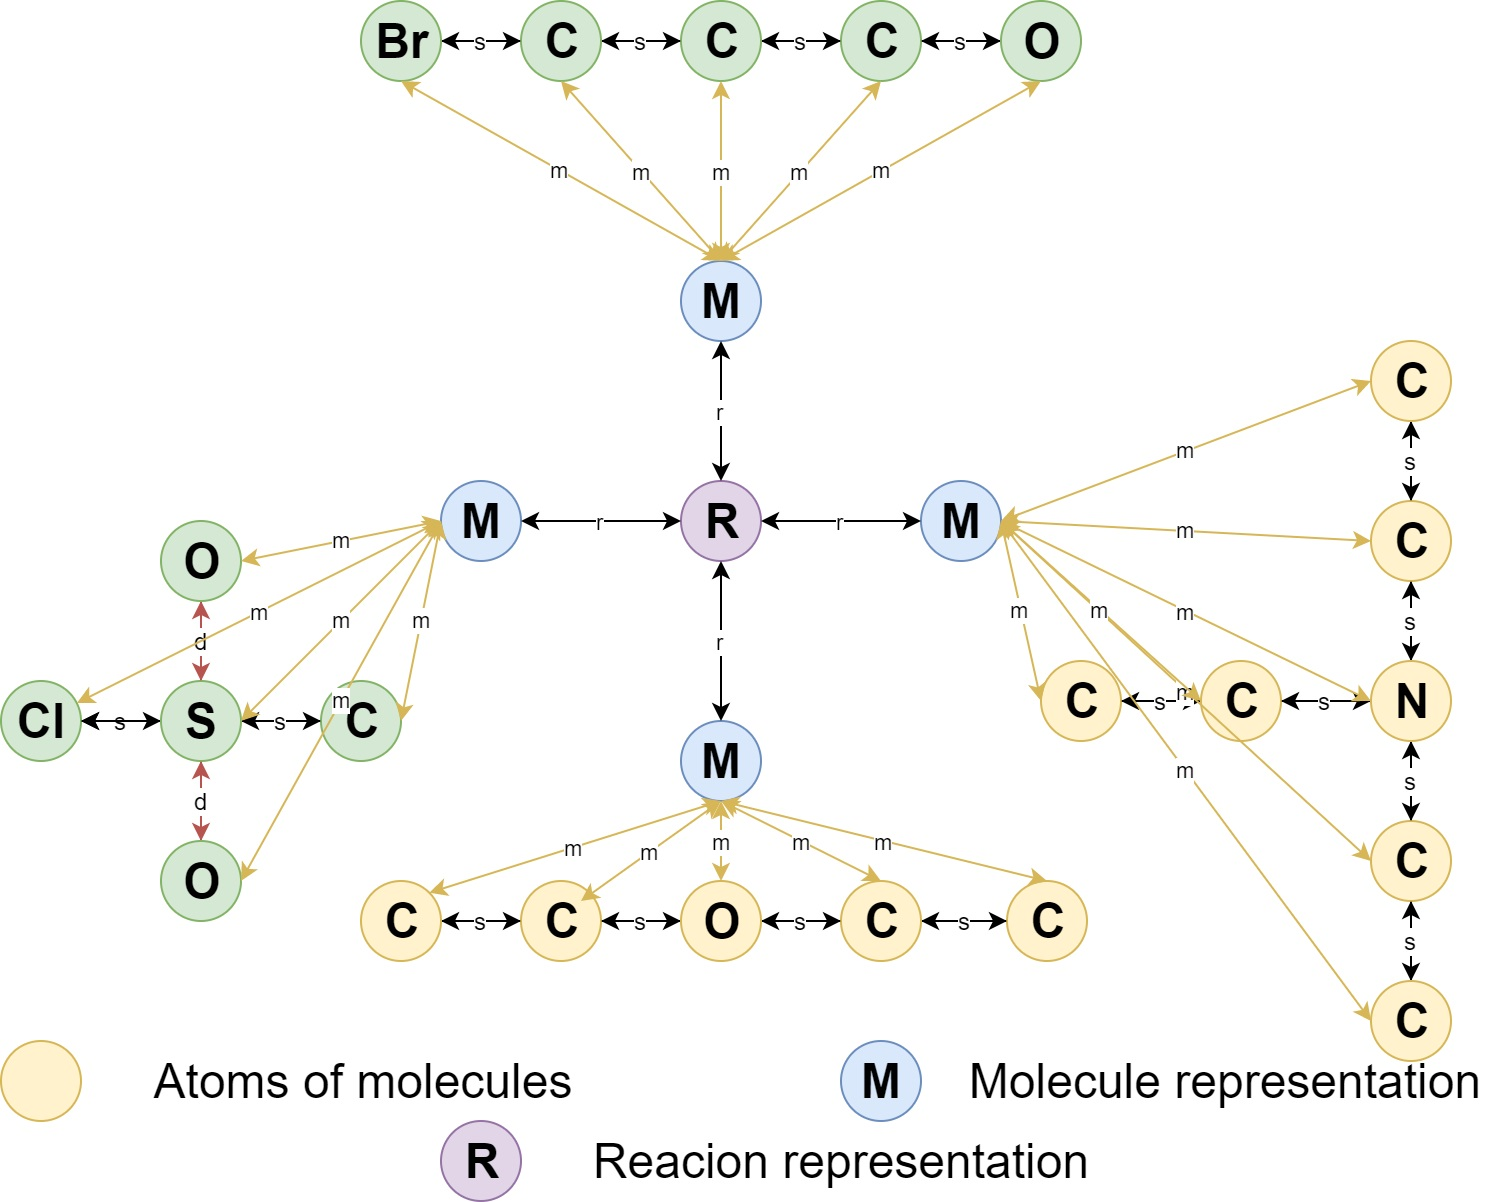
\includegraphics[width=0.8\textwidth]{supernode(1).jpg}
    \caption{\footnotesize{Расширенный граф с введенными вершинами~--- представлениями молекул и реакции.}}


    
\end{frame}

\begin{frame}{Полносвязная сеть}

\begin{block}{Агрегация графа}
$$
\mathbf{h}_g = \dfrac{1}{n}\sum_{i = 1}^n \mathbf{h}_{i = 1}^{(m)},
$$
$\mathbf{h}_g$ -- векторное представление расширенного графа, $m$ -- число слоев RGCNN.
\end{block}
\begin{block}{FCNN}
\centering
\begin{aligned}
    &\mathbf{h}^{(l+1)}_g = \text{ReLU}(\text{linear}(\mathbf{h}_g^{(l)})),\\
    &\hat{y} = \text{linear}({\mathbf{h}^{(t)}_g}), ~\hat{y}\text{ -- выход сети.}
    \label{eq:fcnn}
\end{aligned}

\end{block}

\begin{block}{Функция ошибки}
$$
\mathcal{L} = \dfrac{1}{N}\sum_{i = 1}^N \|y - \hat{y}\|_2^2, ~y\text{ -- реальный выход реакции.}
$$
\end{block}
\end{frame}



\begin{frame}{Вычислительный эксперимент}

\begin{block}{Цели эксперимента}
\begin{enumerate}
    \item Проверить, повышается ли качество модели при последовательном добавлении дополнительной информации о структуре графа.
    \item Может ли предлагаемая модель давать более высокое качество, чем константная модель.
\end{enumerate}

\end{block}

\begin{block}{Эксперименты}

\begin{enumerate}
    \item \textbf{CONST} -- константная модель,
    \item \textbf{BASE} -- базовая модель(RGCNN + FCNN),
    \item \textbf{EG} -- модель расширенного графа,
    \item \textbf{EGB} -- модель с различными типами химической связи,
    \item \textbf{EGBF} -- модель с дополнительной информацией о свойтсвах атомов.
\end{enumerate}

\end{block}


\end{frame}
%----------------------------------------------------------------------------------------------------------
\begin{frame}{Результаты экспериментов}

\begin{multicols}
\normalsize
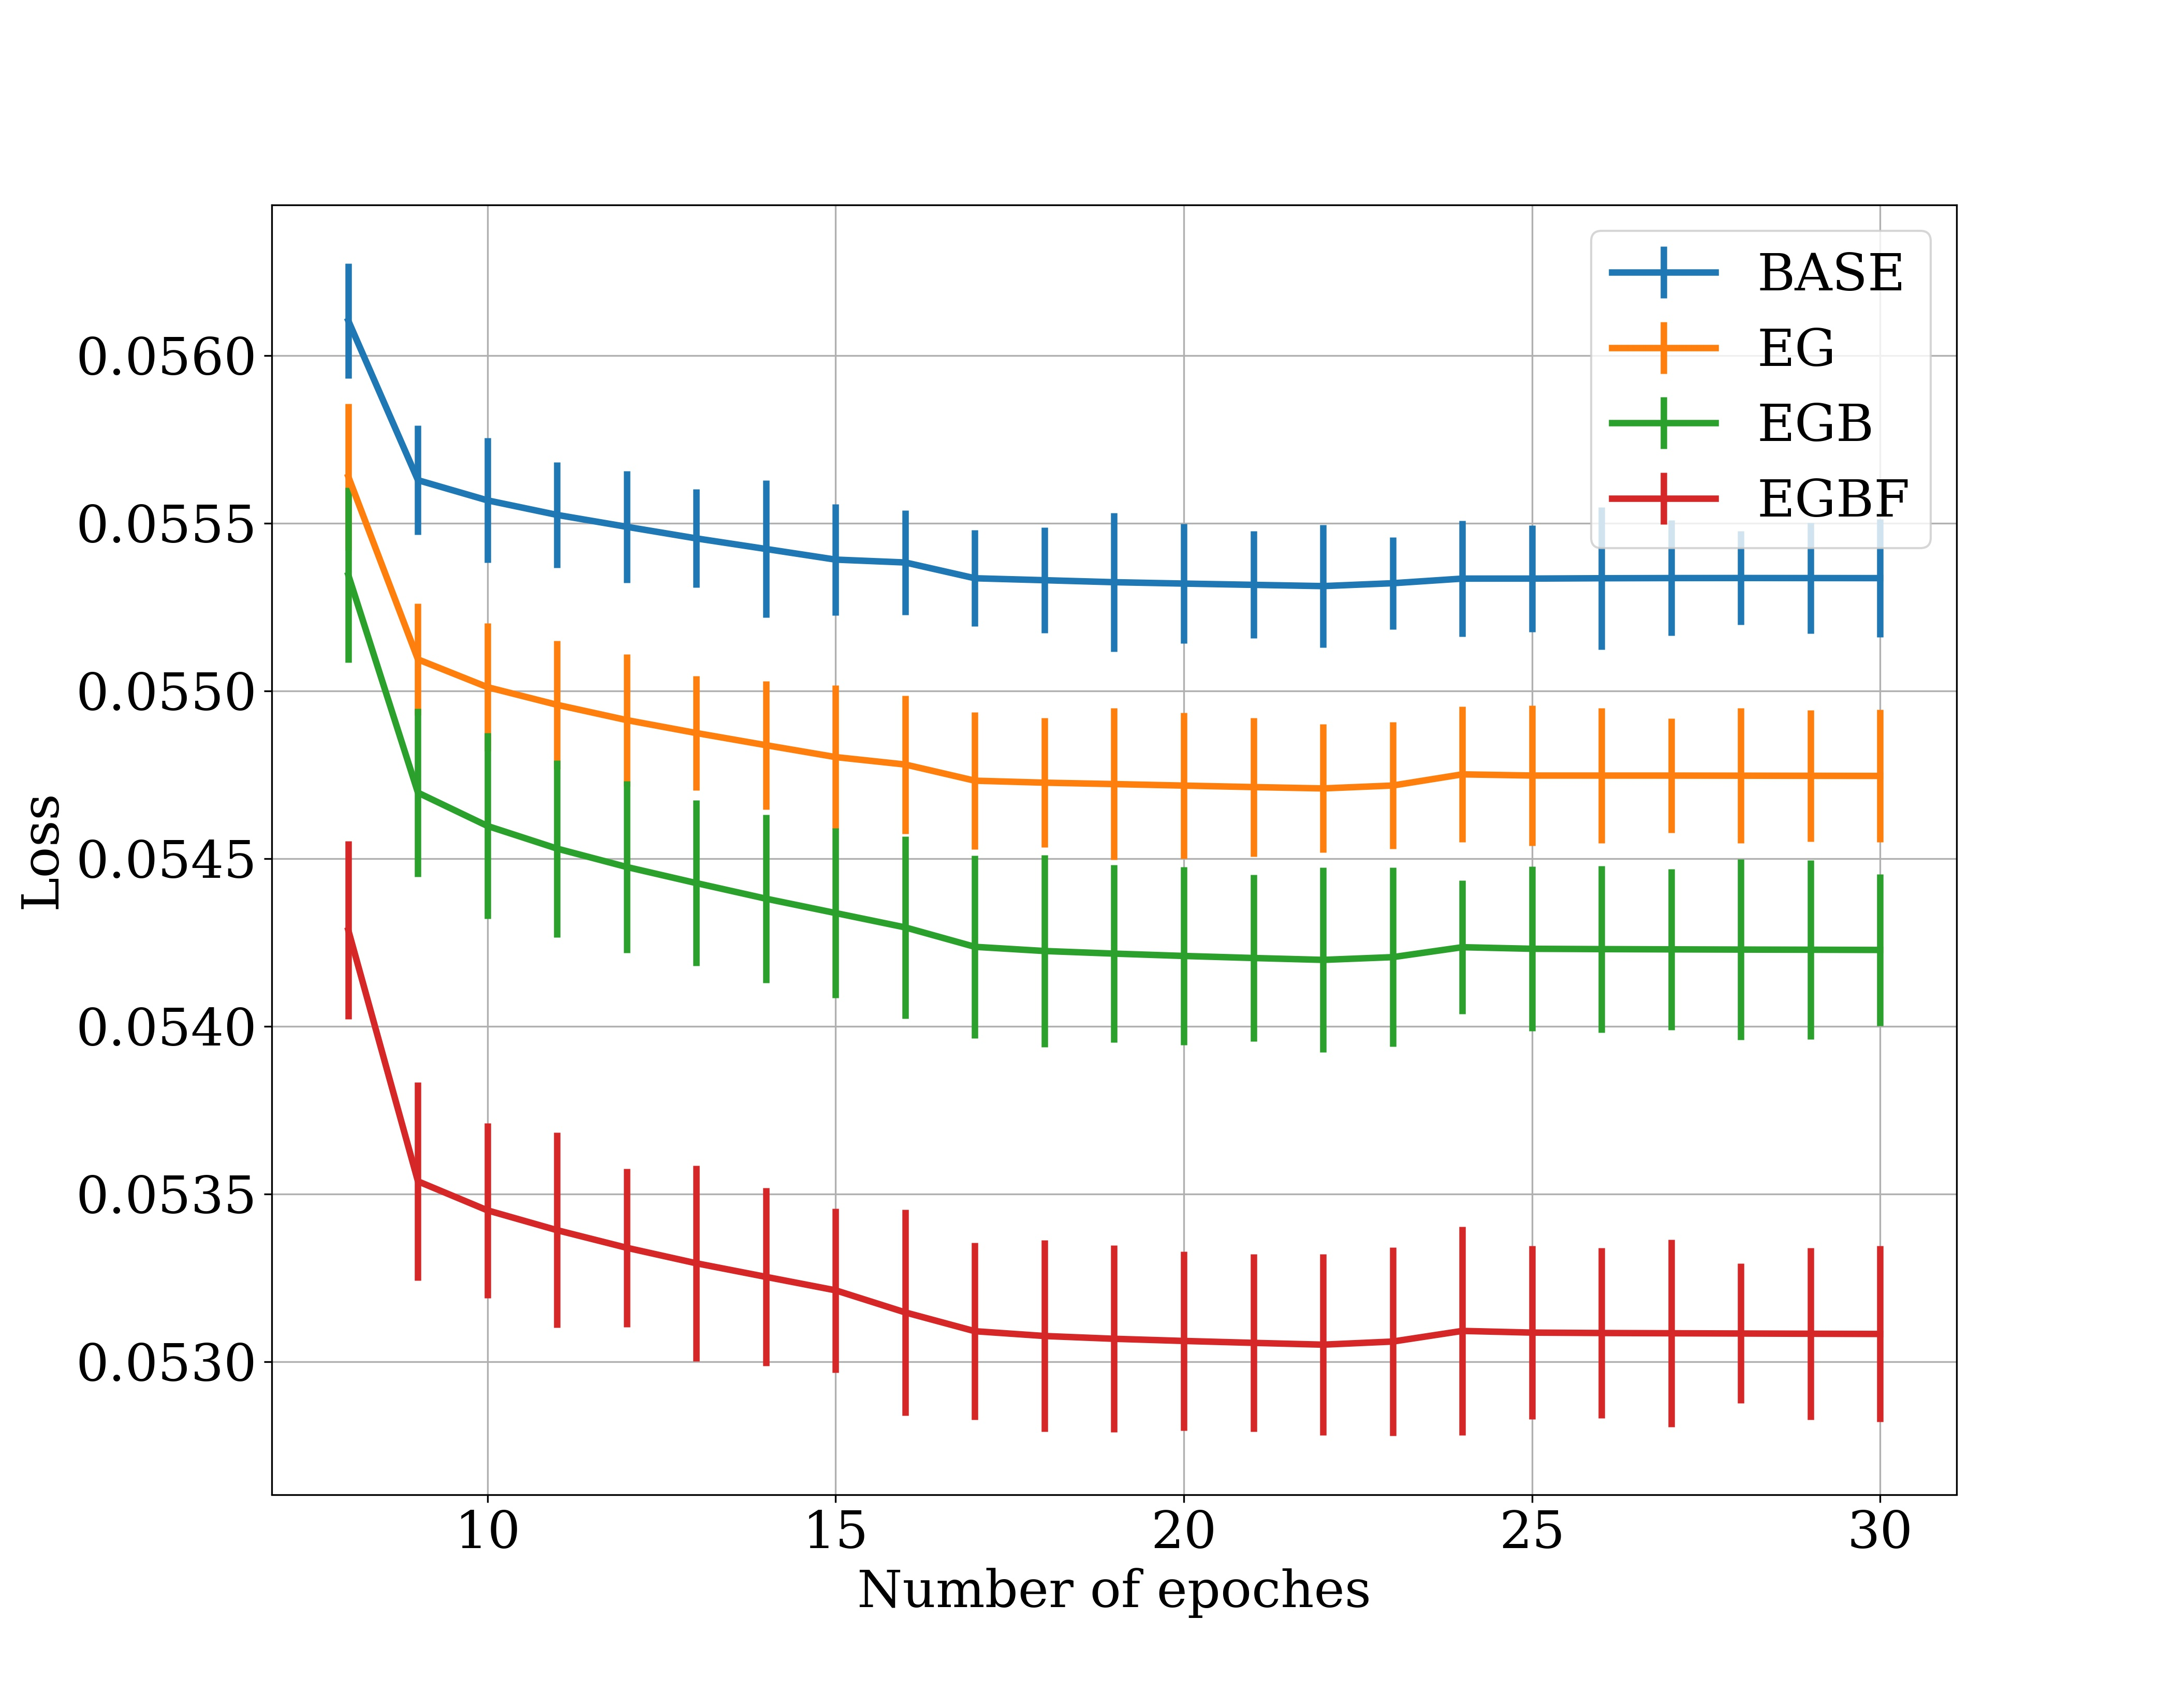
\includegraphics[width=0.58\textwidth]{com_graph(2).jpg}
\centering
\caption{\footnotesize{Ошибка во время обучения}}
\columnbreak

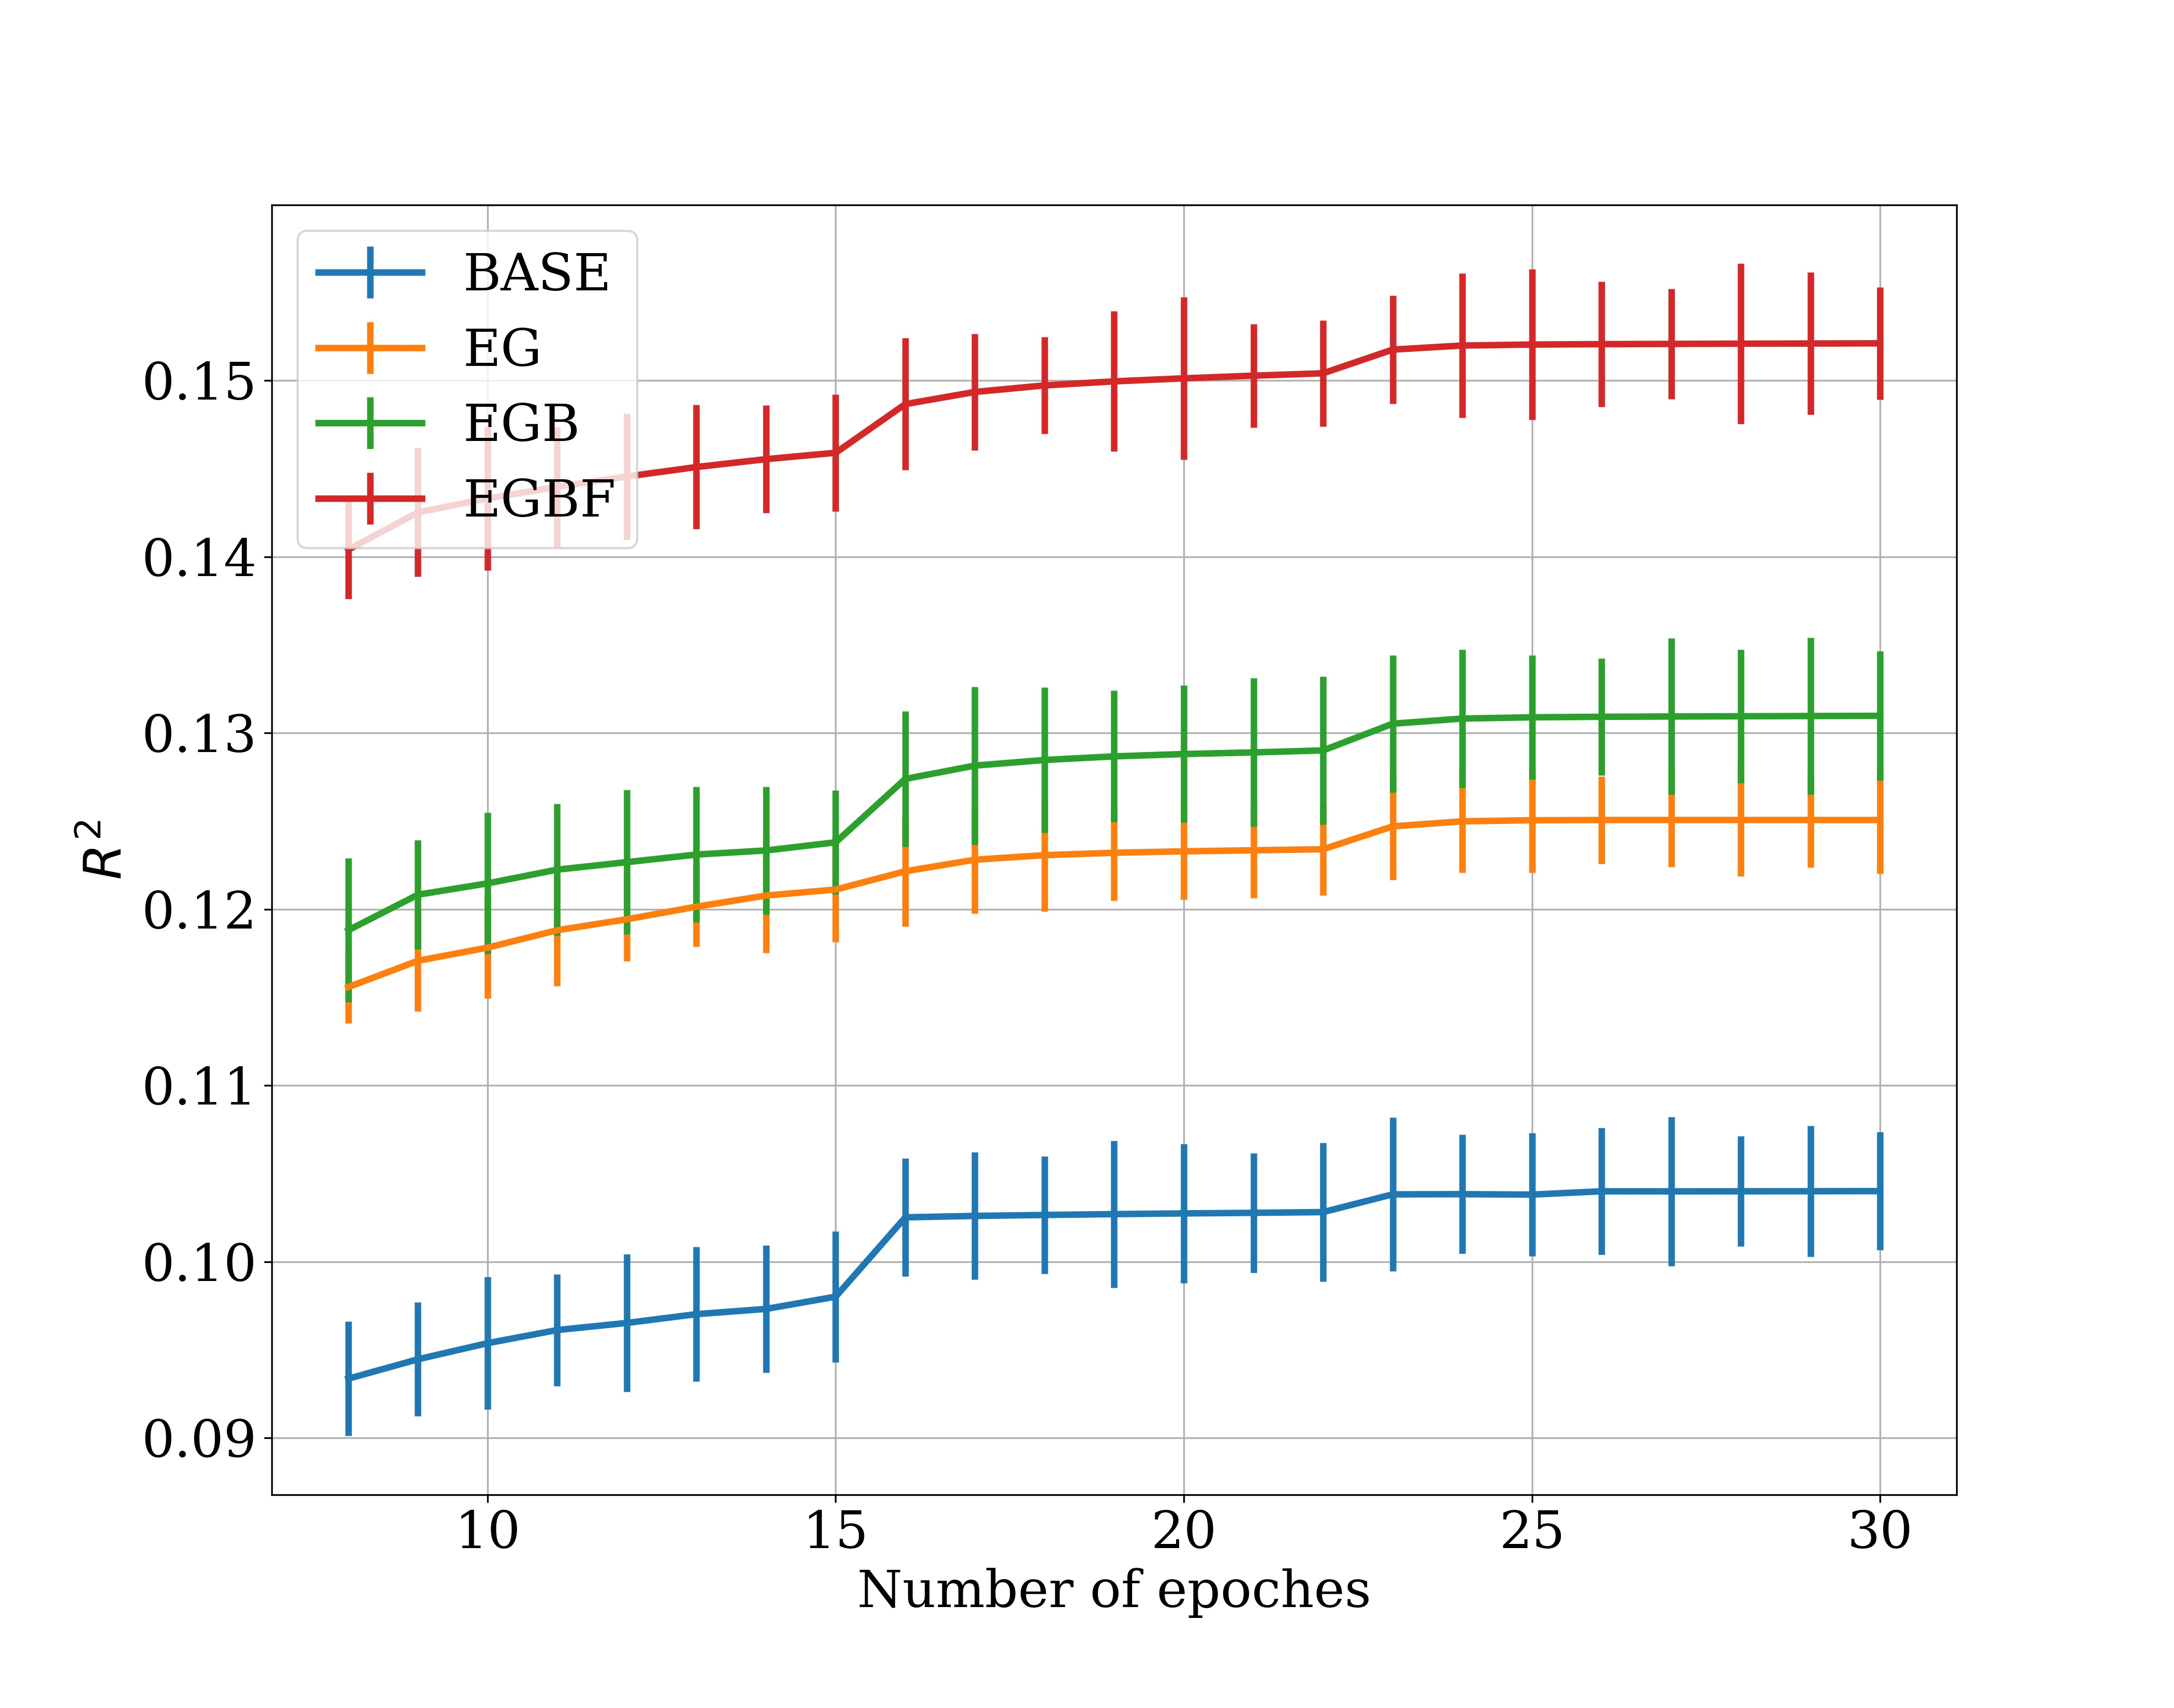
\includegraphics[width=0.58\textwidth]{com_graph_r2(2).jpg}
\centering
\caption{\footnotesize{$R^2$ для тестовой выборки}}
\end{multicols}

При каждой модификации архитектуры уменьшаются ошибки во время обучения и повышается качество на тестовой выборке.

\end{frame}

\begin{frame}{Вывод}
\begin{block}{}

\begin{center}
\begin{tabular}{|c|c|c|}
\hline
& \multicolumn{2}{c|}{\textbf{Mined Yield}} \\
\cline{2-3}
\raisebox{1.5ex}[0cm][0cm]{Модель}
& $R^2$ & $MAE$ \\
\hline
\textbf{CONST} & $0$ & $0.211 \pm 0.004$\\
\hline
\textbf{BASE} & $0.104 \pm 0.002$ & $0.198 \pm 0.003$ \\
\hline
\textbf{EG} & $0.125 \pm 0.003$ & $0.194 \pm 0.002$\\
\hline
\textbf{EGB} & $0.131 \pm 0.006$ & $0.186 \pm 0.002$\\
\hline
\textbf{EGBF} & $0.152 \pm 0.005$ & $0.174 \pm 0.003$\\
\hline
\end{tabular}
\end{center}
\caption{\footnotesize{$R^2$ -- коэффициент детерминации. $MAE$ -- среднее абсолютное отклонение между реальными выходами реакций и предсказанными на тестовой выборке.} }
\end{block}
Каждая из предложенных моделей показала более высокое качество чем константная модель. Самое высокое качество наблюдается у модели \textbf{EGBF}.


\end{frame}


\begin{frame}{Заключение}
    \begin{block}{Полученные результаты}
    \begin{enumerate}
        \item При добавлении дополнительной информации о структуре графа качество модели повысилось.
        \item Предложенная модель показала более высокое качество, чем константная модель.
    \end{enumerate}
    \end{block}
    \begin{block}{Дальнейшие исследования}
    \begin{enumerate}
        \item Классификация типов реакций для повышения качества регрессии.
        \item Определение влияния свойств атомов на качество предложенной модели.
    \end{enumerate}
    \end{block}
\end{frame}
%----------------------------------------------------------------------------------------------------------


\end{document} 